\documentclass[a4paper, 12pt]{ctexart}

% 页边距设置为上下左右各 1.2cm
\usepackage{geometry}
\geometry{left=1.2cm, right=1.2cm, top=1.2cm, bottom=1.2cm}

% 数学宏包
\usepackage{amsmath}
\usepackage{amssymb}

% 颜色与图层宏包
\usepackage{xcolor}
\usepackage{tikz}

% 全局去掉默认页码
\pagestyle{empty}

% ==================== 图层技术实现 ====================

% 1. 在底层（背景层）铺满行距 0.9cm 的灰色横线
\AddToHook{shipout/background}{%
    \begin{tikzpicture}[remember picture, overlay]
        % A4纸高 29.7cm，上下边距 1.2cm，可用高度 27.3cm。27.3 / 0.9 = 30.33
        \foreach \i in {1,...,30} {
            \draw[gray, line width=0.4pt]
                ([xshift=1.2cm, yshift=-1.2cm - \i*0.9cm]current page.north west) --
                ([xshift=-1.2cm, yshift=-1.2cm - \i*0.9cm]current page.north east);
        }
    \end{tikzpicture}%
}

% 2. 在顶层（前景层）添加页码，绝对定位，不干扰正文
\AddToHook{shipout/foreground}{%
    \begin{tikzpicture}[remember picture, overlay]
        \node at ([yshift=1cm]current page.south) {\thepage};
    \end{tikzpicture}%
}

% 3. 定义带纯白背景的题干容器，用于遮挡底层的横线
\setlength{\fboxsep}{5pt}
\newcommand{\whitebox}[1]{%
    \noindent\colorbox{white}{%
        \parbox{\dimexpr\textwidth-2\fboxsep\relax}{#1}%
    }%
}
% ======================================================

\begin{document}
\zihao{-4}

% ==================== 第 1 页（共 2 题） ====================
% 14.2
\noindent
\begin{minipage}[t][0.48\textheight]{\textwidth}
    \whitebox{%
        \textbf{14.2}\quad 设一物体沿 $x$ 轴做简谐振动，振幅为 $12\ \mathrm{cm}$，周期为 $2.0\ \mathrm{s}$，在 $t=0$ 时位移为 $6.0\ \mathrm{cm}$ 且向 $x$ 轴正方向运动。试求：
        \par
        （1）初相位；
        \par
        （2）$t=0.5\ \mathrm{s}$ 时该物体的位置、速度和加速度；
        \par
        （3）在 $x=-6.0\ \mathrm{cm}$ 且向 $x$ 轴负方向运动时，物体的速度、加速度以及它从这个位置到达平衡位置所需要的最短时间。
    }
\end{minipage}

\vspace{0.3cm}

% 14.4
\noindent
\begin{minipage}[t][0.48\textheight]{\textwidth}
    \whitebox{%
        \textbf{14.4}\quad 两质点沿同一直线做频率和振幅均相同的简谐振动，当它们每次沿相反方向互相通过时，它们的位移均为它们振幅的一半，求这两个质点振动的相位差。
    }
\end{minipage}

\newpage

% ==================== 第 2 页（共 2 题） ====================
% 14.5 + 图 14-47
\noindent
\begin{minipage}[t][0.48\textheight]{\textwidth}
    \whitebox{%
        \textbf{14.5}\quad 一简谐振动如图 14-47 所示，已知速度振幅为
        $10\ \mathrm{cm}\cdot\mathrm{s}^{-1}$，求振动方程。
        \par\smallskip
        \begin{center}
        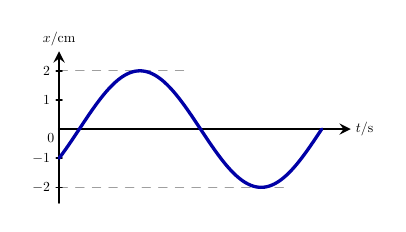
\begin{tikzpicture}[x=0.98cm,y=0.74cm,scale=0.5,transform shape,>=stealth,line cap=round]
            % 位移—时间坐标轴
            \draw[->,line width=0.8pt] (0,-2.53) -- (0,2.67)
                node[above] {$x/\mathrm{cm}$};
            \draw[->,line width=0.8pt] (0,0) -- (7.56,0)
                node[right] {$t/\mathrm{s}$};
            % 振幅辅助线、坐标标记
            \draw[dashed,gray!75] (0,2) -- (3.35,2);
            \draw[dashed,gray!75] (0,-2) -- (6.0,-2);
            \foreach \v in {-2,-1,1,2} {
                \draw[line width=0.55pt] (-0.075,\v) -- (0.075,\v);
                \node[left] at (-0.11,\v) {$\v$};
            }
            \node[below left] at (0,0) {$0$};
            % x(0)=-1 cm，初始上行；曲线仅作原图示意
            \draw[very thick,blue!65!black,samples=130,domain=0:6.8068]
                plot (\x,{2*sin(deg(\x)-30)});
        \end{tikzpicture}
        \par\smallskip {\small 图 14-47\quad 习题 14.5 图}
        \end{center}
    }
\end{minipage}

\vspace{0.3cm}

% 14.9 + 图 14-49（上：双侧并联效果；下：两弹簧串联）
\noindent
\begin{minipage}[t][0.48\textheight]{\textwidth}
    \whitebox{%
        \textbf{14.9}\quad 用弹性系数分别为 $k_1$ 和 $k_2$ 的两个弹簧以及质量为 $m$ 的物体，在光滑的桌面上分别构成如图 14-49 所示的两种振子，求这两个系统的固有角频率。
        \par\smallskip
        \begin{center}
        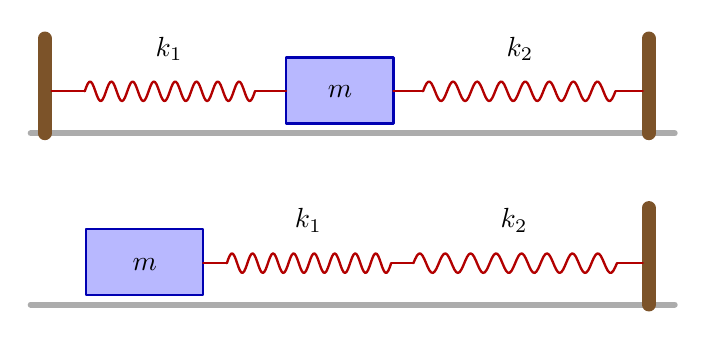
\begin{tikzpicture}[x=0.94cm,y=0.73cm,line join=round,line cap=round]
            % 图 (a)：质量块两侧各连一弹簧
            \draw[gray!65,line width=2.2pt] (0.15,3.45) -- (8.85,3.45);
            \draw[brown!65!black,line width=5pt] (0.34,3.45) -- (0.34,5.10);
            \draw[brown!65!black,line width=5pt] (8.50,3.45) -- (8.50,5.10);
            \filldraw[fill=blue!28,draw=blue!70!black,line width=0.8pt]
                (3.60,3.62) rectangle (5.05,4.77);
            \node at (4.33,4.17) {$m$};
            \draw[red!70!black,line width=0.85pt] (0.43,4.18) -- (0.88,4.18);
            \draw[red!70!black,line width=0.85pt,samples=115,domain=0.88:3.18]
                plot (\x,{4.18+0.17*sin(360*8*(\x-0.88)/2.30)});
            \draw[red!70!black,line width=0.85pt] (3.18,4.18) -- (3.60,4.18);
            \draw[red!70!black,line width=0.85pt] (5.05,4.18) -- (5.45,4.18);
            \draw[red!70!black,line width=0.85pt,samples=115,domain=5.45:8.05]
                plot (\x,{4.18+0.17*sin(360*8*(\x-5.45)/2.60)});
            \draw[red!70!black,line width=0.85pt] (8.05,4.18) -- (8.42,4.18);
            \node[above] at (2.02,4.55) {$k_1$};
            \node[above] at (6.76,4.55) {$k_2$};
            % 图 (b)：两只弹簧串联后连接右侧固定端
            \draw[gray!65,line width=2.2pt] (0.15,0.47) -- (8.85,0.47);
            \draw[brown!65!black,line width=5pt] (8.50,0.47) -- (8.50,2.15);
            \filldraw[fill=blue!28,draw=blue!70!black,line width=0.8pt]
                (0.90,0.64) rectangle (2.48,1.79);
            \node at (1.69,1.17) {$m$};
            \draw[red!70!black,line width=0.85pt] (2.48,1.19) -- (2.80,1.19);
            \draw[red!70!black,line width=0.85pt,samples=115,domain=2.80:5.02]
                plot (\x,{1.19+0.17*sin(360*8*(\x-2.80)/2.22)});
            \draw[red!70!black,line width=0.85pt] (5.02,1.19) -- (5.32,1.19);
            \draw[red!70!black,line width=0.85pt,samples=115,domain=5.32:8.07]
                plot (\x,{1.19+0.17*sin(360*8*(\x-5.32)/2.75)});
            \draw[red!70!black,line width=0.85pt] (8.07,1.19) -- (8.42,1.19);
            \node[above] at (3.90,1.56) {$k_1$};
            \node[above] at (6.68,1.56) {$k_2$};
        \end{tikzpicture}
        \par\smallskip {\small 图 14-49\quad 习题 14.9 图}
        \end{center}
    }
\end{minipage}

\newpage

% ==================== 第 3 页（共 2 题） ====================
% 14.20
\noindent
\begin{minipage}[t][0.48\textheight]{\textwidth}
    \whitebox{%
        \textbf{14.20}\quad 一质点同时参与同一直线上的两个简谐振动
        $\sqrt{3}\cos\!\left(\omega t+\dfrac{\pi}{2}\right)$（SI 单位）和
        $\cos\omega t$。试求该质点的合振动的振幅 $A$ 及初相位 $\varphi_0$。
    }
\end{minipage}

\vspace{0.3cm}

% 14.23 + 图 14-56
\noindent
\begin{minipage}[t][0.48\textheight]{\textwidth}
    \whitebox{%
        \textbf{14.23}\quad 图 14-56 所示为两个同振幅、同频率简谐振动，写出它们的合振动的表达式。
        \par\smallskip
        \begin{center}
        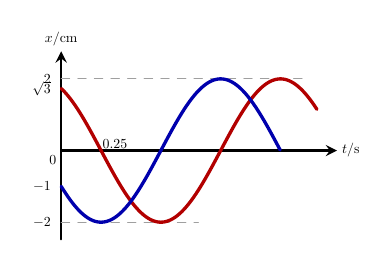
\begin{tikzpicture}[x=4.05cm,y=0.91cm,scale=0.5,transform shape,>=stealth,line cap=round]
            % 两曲线振幅均为 2 cm；沿同一时间轴绘出
            \draw[->,line width=0.8pt] (0,-2.48) -- (0,2.77)
                node[above] {$x/\mathrm{cm}$};
            \draw[->,line width=0.8pt] (0,0) -- (1.73,0)
                node[right] {$t/\mathrm{s}$};
            \draw[gray!75,dashed] (0,2) -- (1.53,2);
            \draw[gray!75,dashed] (0,-2) -- (0.86,-2);
            \node[left] at (-0.035,2) {$2$};
            \node[left] at (-0.035,1.732) {$\sqrt{3}$};
            \node[left] at (-0.035,-1) {$-1$};
            \node[left] at (-0.035,-2) {$-2$};
            \node[below left] at (0,0) {$0$};
            % 14-56 原图给出 t=0.25 s（红线第一次向下过零）
            \node[above right,inner sep=1pt] at (0.25,0) {$0.25$};
            % 红线：x(0)=sqrt(3) cm，初始负向；同频率同振幅
            \draw[very thick,red!70!black,samples=160,domain=0:1.605]
                plot (\x,{2*cos(240*\x+30)});
            % 蓝线：x(0)=-1 cm，初始负向
            \draw[very thick,blue!68!black,samples=160,domain=0:1.375]
                plot (\x,{2*cos(240*\x+120)});
        \end{tikzpicture}
        \par\smallskip {\small 图 14-56\quad 习题 14.23 图}
        \end{center}
    }
\end{minipage}

\end{document}
